\documentclass[a4paper,12pt]{article}
\usepackage{polski}
\usepackage[utf8]{inputenc}
\usepackage[left = 3cm, right = 3cm, top = 2cm, bottom = 2cm]{geometry}
\usepackage{enumerate}
\usepackage{amssymb}		% pakiet do symboli
\usepackage{amsmath}		% pakiet do matmy
\usepackage{enumitem}		% punktowanie (a), (b), ...
\usepackage{nopageno}		% brak numerow stron
\usepackage{graphicx}		% wstawianie obrazkow
\usepackage{float}			% wstawianie obrazkow w dowolnym miejscu
\usepackage{titling}
%\usepackage[]{algorithm2e} 	% algorytmy :))
\usepackage{algpseudocode}	
%\usepackage{program}
%\usepackage{algorithmicx}
\usepackage{algorithm}

% nowe komendy dla wygodniejszego pisania :)
\newcommand{\subtitle}[1]{ \posttitle{ \par\end{center} \begin{center}\large#1\end{center} \vskip0.5em}}
\newcommand{\floor}[1]{\left\lfloor #1 \right\rfloor}
\newcommand{\ceil}[1]{\left\lceil #1 \right\rceil}
\newcommand{\code}[1]{\fontfamily{qcr}\selectfont\textbf{#1}\fontfamily{cmr}\selectfont}

\begin{document}
\noindent \textbf{Lista 4, zadanie 8 - Tomasz Woszczyński}\newline

\noindent \newline \textbf{Treść:} Na każdym polu szachownicy o wymiarach $4 \times n$ znajduje się jedna liczba naturalna. Ułóż algorytm, który umieszcza na szachownicy kamyki w taki sposób, że:
\begin{itemize}
\item na każdym polu znajduje się co najwyżej jeden kamień,
\item jeśli na polu $P$ znajduje się kamyk, to na polach mających wspólny bok z $P$ nie ma kamyków,
\item suma liczb z pól, na których leżą kamyki jest maksymalna.
\end{itemize}

\noindent \textbf{Rozwiązanie:} Rozpatrzmy najpierw jak mogą być ustawione kamyki w poszczególnych kolumnach (numery na dole oznaczają kolejne możliwości, tabelka nie przedstawia też przykładowej z treści zadania):

\begin{figure}[H]
\centering
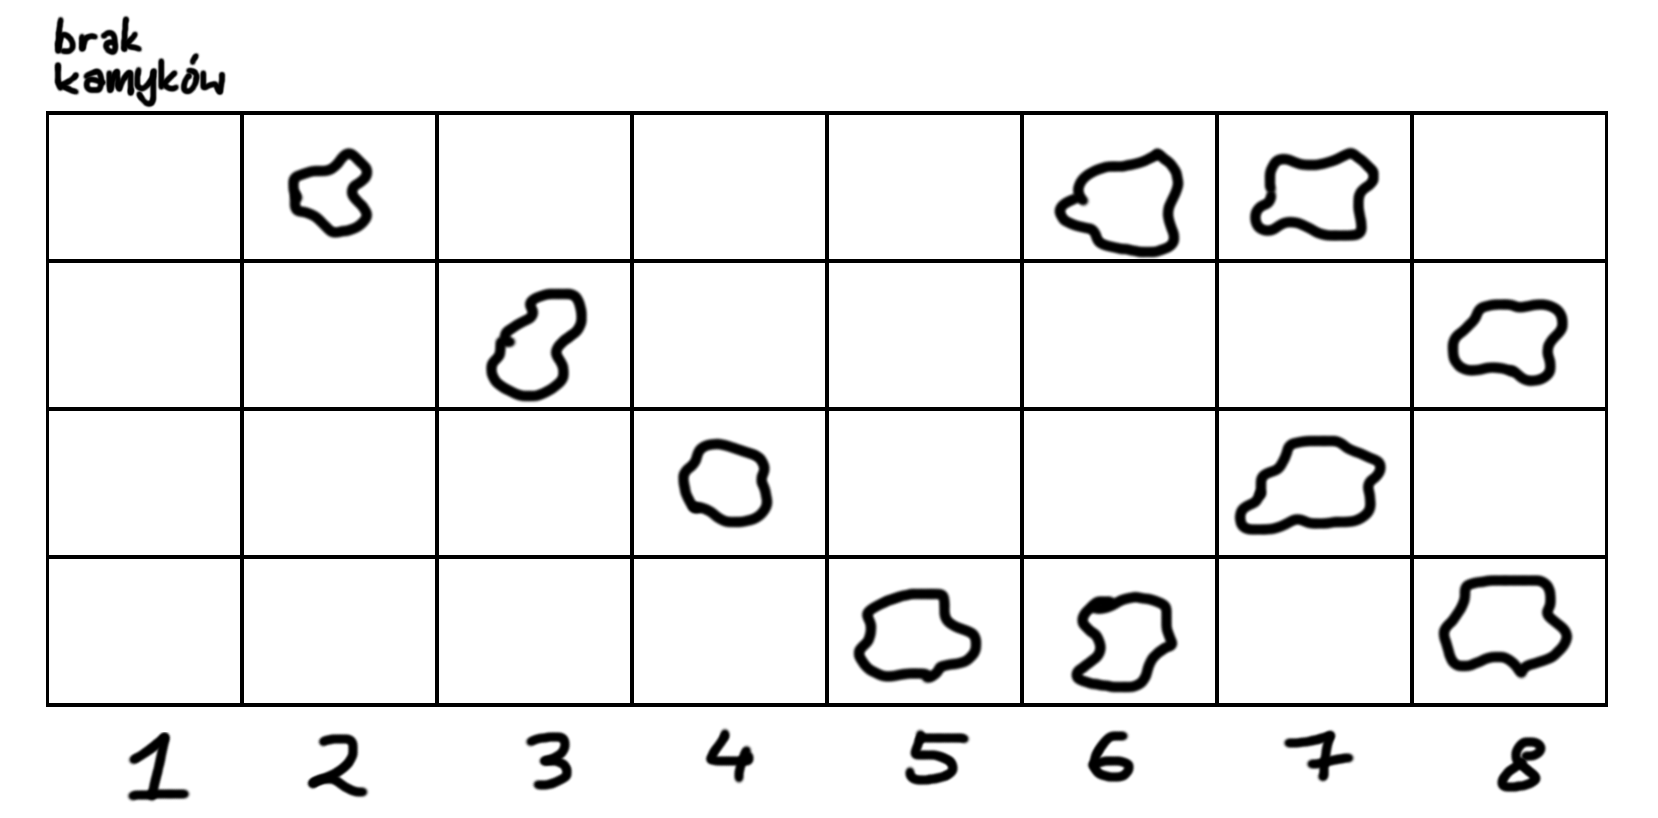
\includegraphics[width=.8\textwidth]{kamyki.png}
\end{figure}

\noindent Zastosowanie każdej z możliwości zależy od wyboru położenia kamieni w poprzedniej kolumnie, oznacza to, że nie możemy mieć w dwóch kolejnych kolumnach niektórych ułożeń kamyków, gdyż nie zgadzało by się to z drugim warunkiem z treści. Oznaczmy sobie przez \code{c[i][j]} sumę pól w \code{i}-tej kolumnie, przy wyborze możliwości \code{j}. Rozpatrzmy teraz jakie możliwe ułożenia będziemy mieli w kolumnie \code{i-1} oraz \code{i}:

\begin{figure}[H]
\centering
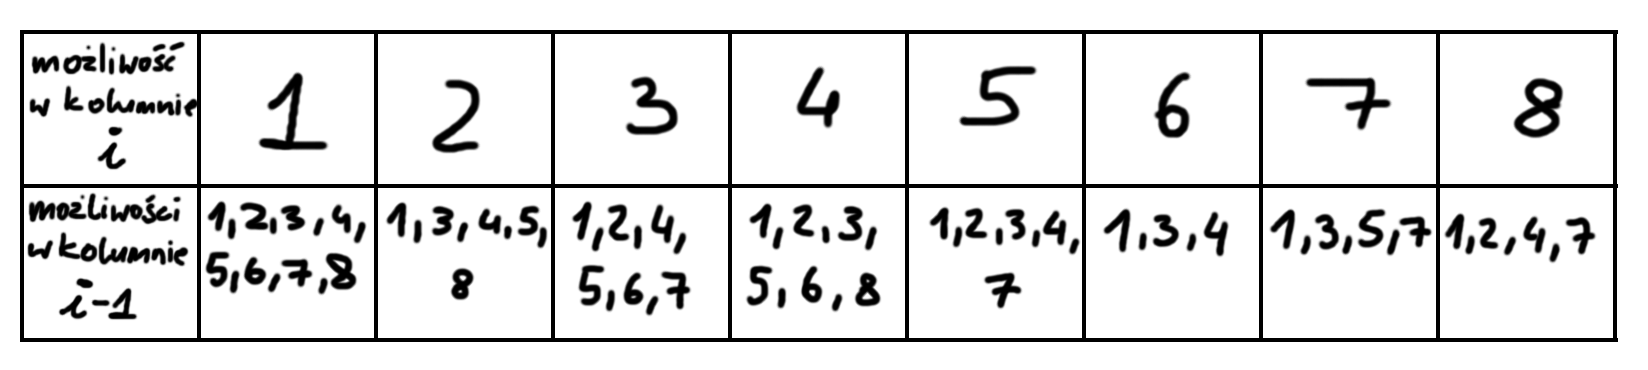
\includegraphics[width=1\textwidth]{kamykitab.png}
\end{figure}

\noindent Zdefiniujemy wtedy funkcję:
$$
\text{\code{T[i][j]}} = \max\limits_{k = \text{\code{mozliwosci(j)}}} \text{\code{(T[i-1][k] + c[i][j])}}
$$
gdzie \code{mozliwosci(x)} zwraca możliwe konfiguracje dla kolumny \code{x}. Algorytm ten wykona się w czasie $O(n)$, gdyż rekurencyjnie przechodzimy przez całą tablicę od ostatniej do pierwszej kolumny i wykona się poprawnie, gdyż za każdym razem dodajemy największą znalezioną wartość z dwóch sąsiednich kolumn. Algorytm działanie zakończy, gdy spełniony będzie warunek \code{i == 0}.

\end{document}